\section{Resultados}
\label{sec:resultados}
\subsection{Panorama nacional das atribuições}

A matriz completa conecta os totais setoriais às relações que os compõem (Figura~\ref{fig:panorama-F}). As cores mostram as atribuições entre cada origem emissora e produto final; as margens somam essas relações pela produção e pela demanda. A diagonal permanece visível, distinguindo a atribuição ao próprio produto das relações entre atividades que serão examinadas na rede externa.

As duas contas totalizam 683,70 mil Gg de CO\textsubscript{2}, dos quais 392,92 mil Gg, ou 57,47\%, ficam na diagonal e 290,78 mil Gg entre atividades distintas. A conservação é uma identidade contábil; a repartição dos pesos é o objeto da análise. Por isso, uma atividade pode concentrar emissões próprias sem distribuir volume semelhante para outros produtos finais.

%TC:ignore
\begin{figure}[!htb]
\centering
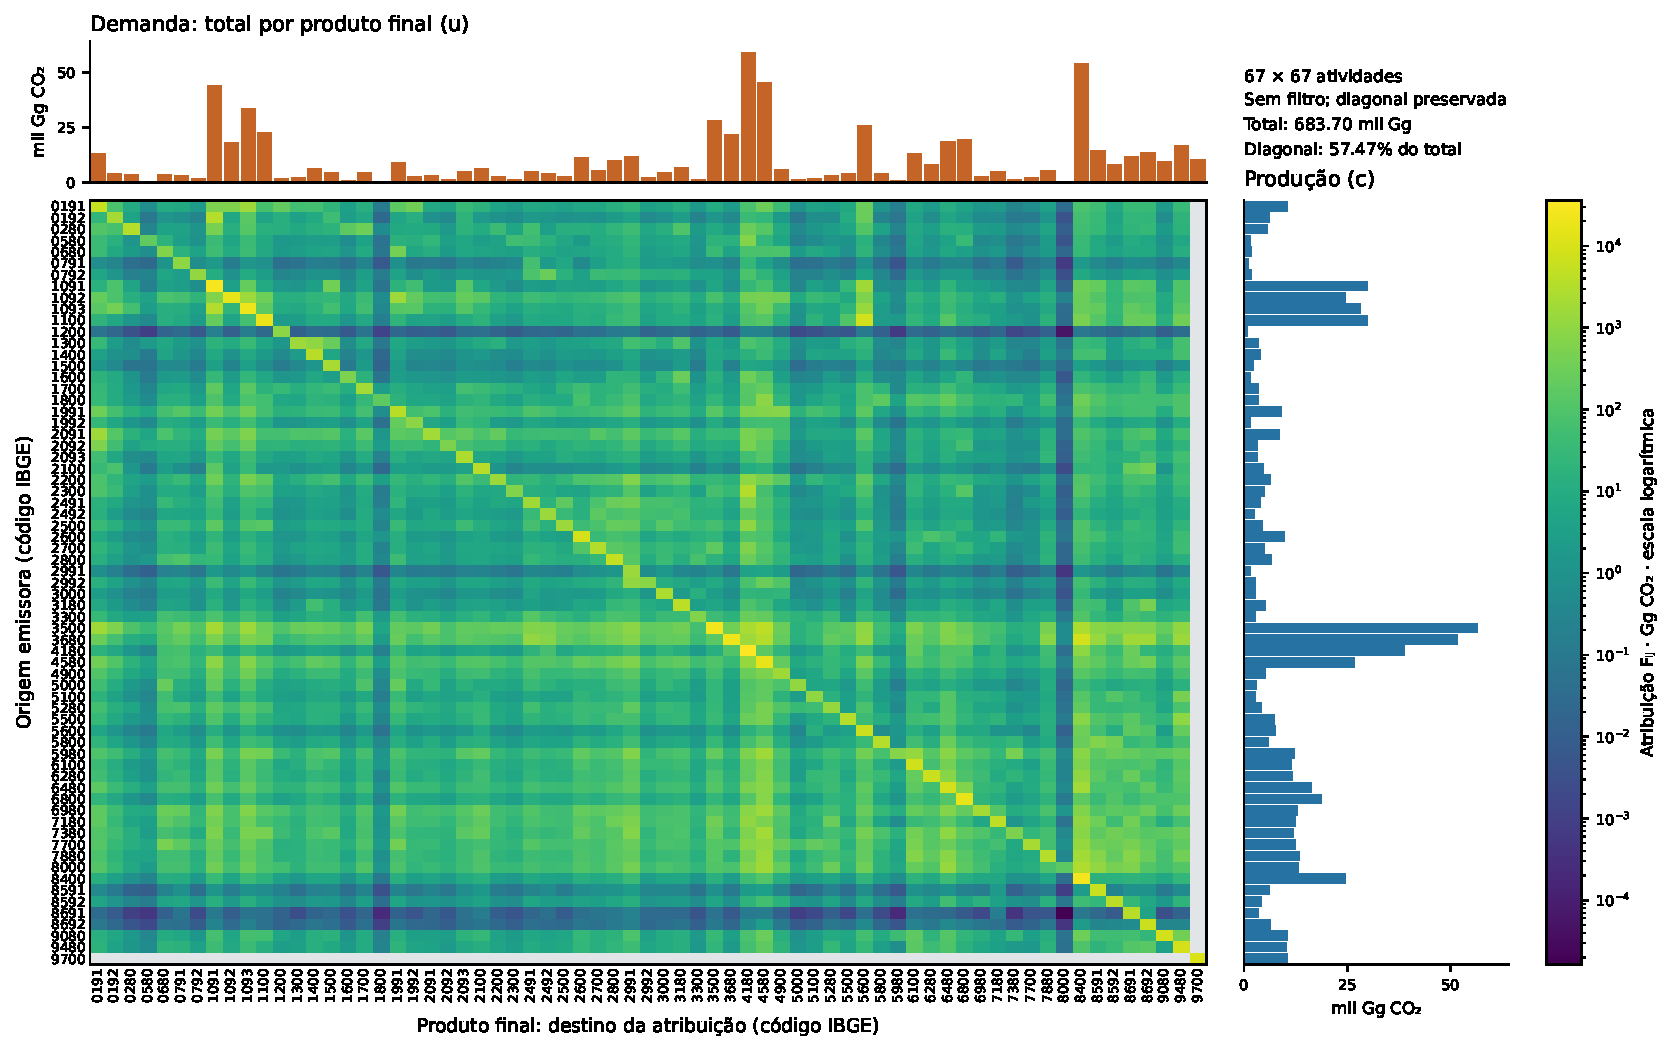
\includegraphics[width=\linewidth,height=0.55\textheight,keepaspectratio]{figuras/artigo_matriz_F.pdf}
\caption{Matriz nacional de atribuição de CO\textsubscript{2} e contas marginais, Brasil, 2015.}
\label{fig:panorama-F}
\begin{minipage}{\linewidth}\footnotesize
Fonte: elaboração própria, MIP do IBGE e intensidades aproximadas de Sanguinet e Azzoni (2024). Matriz $F$ integral: 67 origens emissoras nas linhas e 67 produtos finais nas colunas, na mesma ordem IBGE (códigos no Apêndice E). Cor em escala logarítmica dos pesos positivos, em Gg de CO\textsubscript{2}; cinza: zero. Não há filtro, agregação ou normalização por linha/coluna. A diagonal é preservada. Acima, soma das colunas ($u$, demanda); à direita, soma das linhas ($c$, produção). Barras em mil Gg, com escala linear de mesma amplitude. As duas contas preservam o mesmo total. As células representam atribuição direta e indireta, não transações imediatas.
\end{minipage}
\end{figure}
%TC:endignore

\subsection{Magnitude ambiental e presença produtiva}

As atividades mudam de posição ambiental sem alterar sua presença como fornecedoras. Na Figura~\ref{fig:emissao-fornecedor}, comércio, refino e transporte terrestre apresentam requerimentos elevados nas cadeias padronizadas; água e resíduos e construção combinam menor presença nessa comparação com participação relevante nas emissões próprias do cenário. Energia reúne participação emissora elevada e requerimentos inferiores aos dos três fornecedores destacados. Emitir muito e participar intensamente das cadeias dos demais produtos são dimensões relacionadas, mas distintas.

A passagem da produção à demanda evidencia o papel de construção como destino da atribuição. Sua participação sobe de 5,68\% para 8,69\%, enquanto a de energia cai de 8,28\% para 4,13\%. Comércio também ganha participação, de 3,91\% para 6,64\%. O deslocamento horizontal mantém a mesma estrutura econômica no eixo vertical: muda o critério aplicado às mesmas emissões. Esses contrastes descrevem o cenário adotado, não uma hierarquia ambiental independente da fonte.

%TC:ignore
\begin{figure}[!htb]
\centering
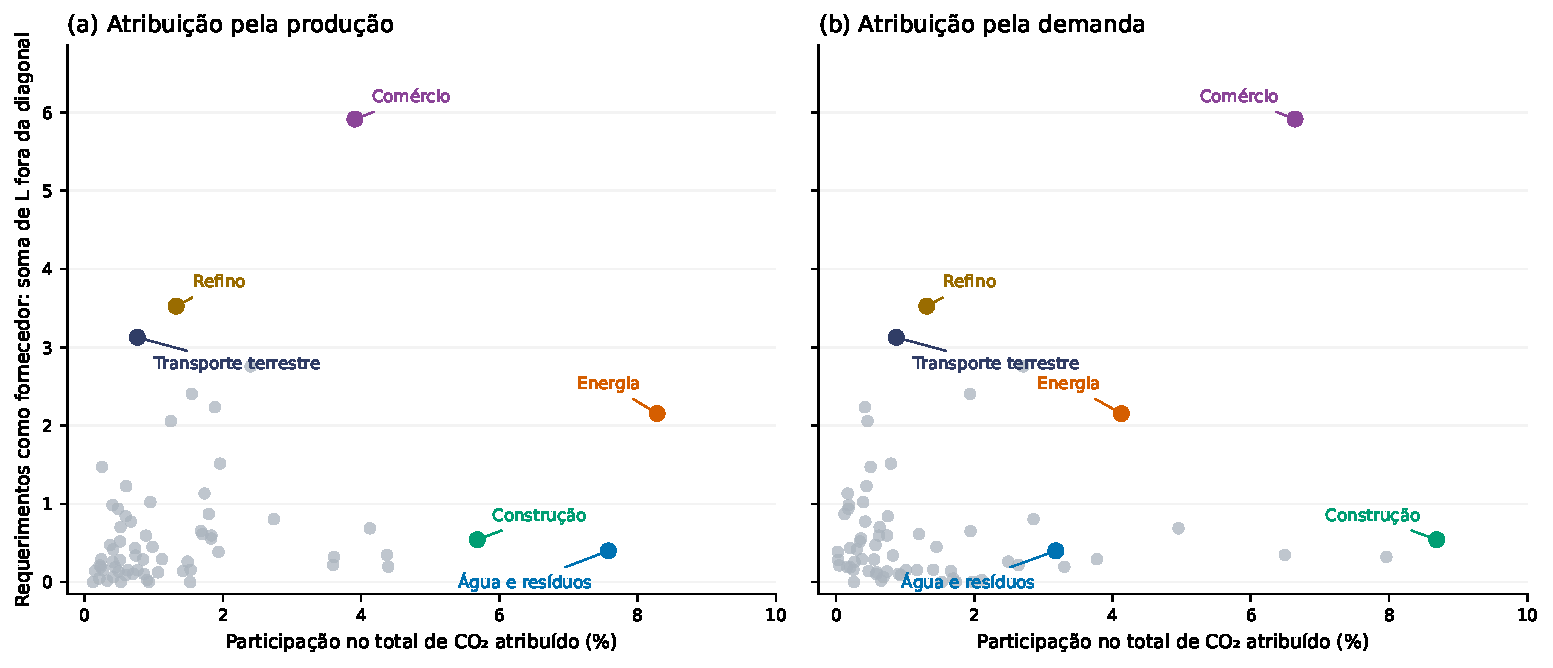
\includegraphics[width=\linewidth,height=0.55\textheight,keepaspectratio]{figuras/emissao_presenca_fornecedor.pdf}
\caption{Presença como fornecedor e participação nas contas pela produção e pela demanda.}
\label{fig:emissao-fornecedor}
\begin{minipage}{\linewidth}\footnotesize
Fonte: elaboração própria, MIP de 2015 e intensidades aproximadas de Sanguinet e Azzoni (2024). Todos os 67 setores, com escalas iguais. Eixo vertical: $q_i=\sum_{j\ne i}L_{ij}$, adimensional, sem diagonal e com peso unitário para cada outro destino. Eixo horizontal: participação percentual em $c$ (a) e $u$ (b), incluindo a diagonal de $F$. Os seis destaques retomam casos explorados anteriormente; não são uma classificação exaustiva. Sem filtragem de ligações.
\end{minipage}
\end{figure}
%TC:endignore

\subsection{Uma rede densa com pesos desiguais}

A rede contém quase todas as conexões possíveis, mas essa presença não descreve a distribuição dos volumes. São 4\,290 arestas, densidade de 97,01\% e 66 atividades conectadas em ambas as direções, com grau 65. Serviços domésticos é o único isolado externo. Os requisitos indiretos incorporados em $F$ contribuem para essa densidade; por isso, contar vínculos positivos pouco distingue os setores.

Os pesos externos se repartem de forma desigual: energia e água/resíduos têm saídas externas próximas, de 31,32 e 31,23 mil Gg, mas 20,79 e 9,88 destinos efetivos. Volumes semelhantes podem, portanto, corresponder a perfis com concentrações diferentes (Figura~\ref{fig:indicadores-resultados}).

O backbone reduz a quantidade de ligações com perdas desiguais de cobertura. Em $\alpha=0{,}05$, preserva 575 arestas, 13,40\% das originais, e 70,69\% do peso intersetorial. Entretanto, as medianas locais são 59,32\% nas saídas e 55,69\% nas entradas, com mínimos próximos de um terço. A cobertura agregada não garante representação igualmente completa de todos os setores. Nos parâmetros 0,01 e 0,10, retêm-se respectivamente 338 e 755 arestas, com 57,39\% e 77,35\% do peso; os detalhes estão no Apêndice~\ref{ap:sensibilidade}.

%TC:ignore
\begin{figure}[!htb]
\centering
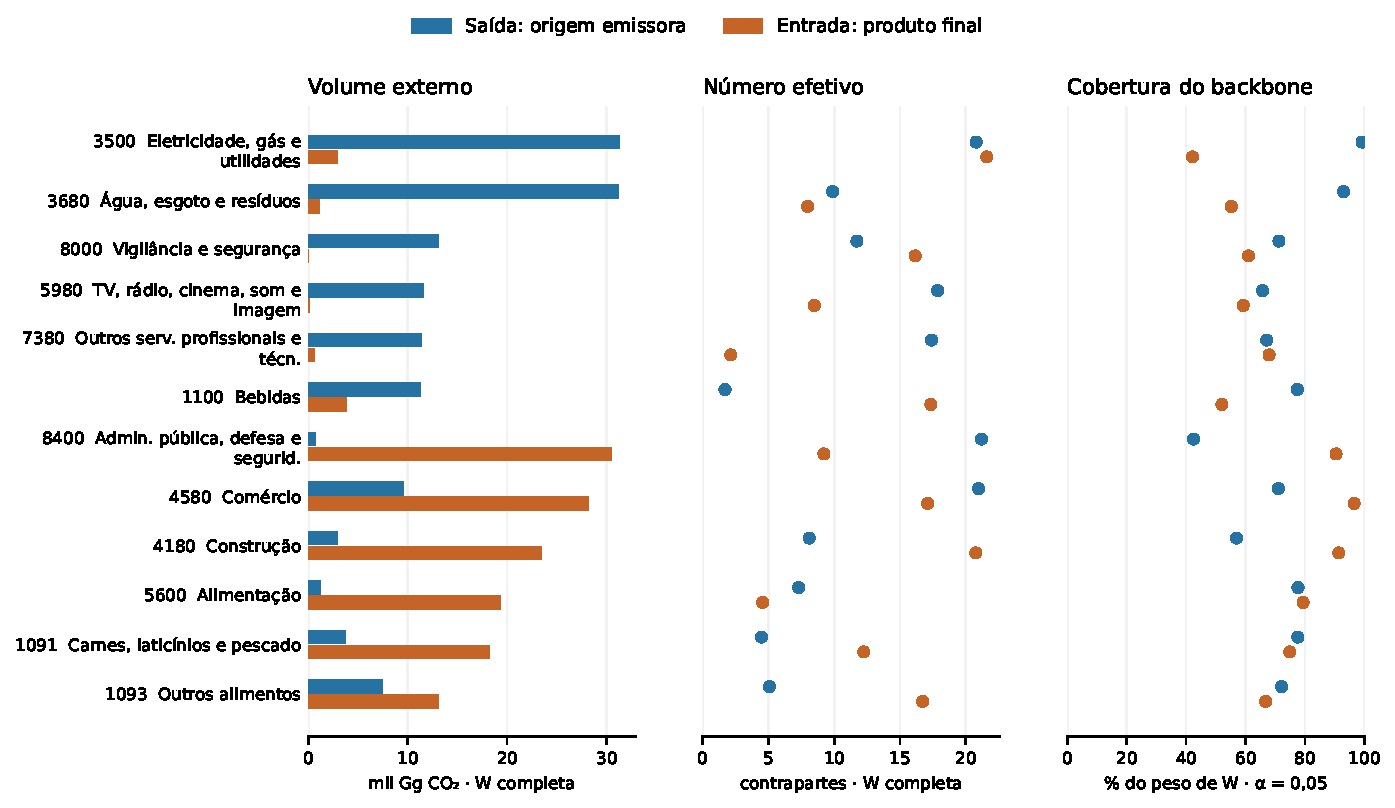
\includegraphics[width=\linewidth,height=0.55\textheight,keepaspectratio]{figuras/artigo_indicadores.pdf}
\caption{Volume, concentração e cobertura descrevem dimensões diferentes.}
\label{fig:indicadores-resultados}
\begin{minipage}{\linewidth}\footnotesize
Fonte: elaboração própria. União das seis maiores forças de saída e seis de entrada em $W$: 12 atividades, na ordem da seleção. Azul: saída da origem emissora; laranja: entrada no produto final. Volume em mil Gg de CO\textsubscript{2} e número efetivo calculados em $W$ completa, sem diagonal. Cobertura: peso retido no backbone de $\alpha=0{,}05$ dividido pela força da mesma atividade e direção. Não é cobertura do inventário ambiental.
\end{minipage}
\end{figure}
%TC:endignore

\subsection{Energia e construção: origens, destinos e contrapartes}

Energia distribui emissões para outros produtos, enquanto construção reúne atribuições de outras origens. Energia tem 56,62 mil Gg pela produção e 28,23 mil Gg pela demanda; suas saídas e entradas externas são 31,32 e 2,92 mil Gg. Construção apresenta 38,84 e 59,40 mil Gg nas contas completas, com 2,93 e 23,48 mil Gg externos. Sua pequena saída externa não significa baixa emissão própria: 35,91 mil Gg permanecem na diagonal.

As contrapartes tornam esses papéis concretos (Figura~\ref{fig:relacoes-focais}). Comércio, administração pública, construção e atividades alimentares aparecem entre os principais destinos externos de energia. Nas entradas de construção destacam-se minerais não metálicos, energia, água/resíduos e comércio. Energia $\rightarrow$ construção representa cerca de 2\,263 Gg, equivalentes a 7,2\% das saídas externas da origem e 9,6\% das entradas externas do destino. A mesma relação tem importância relativa diferente conforme a ponta examinada.

A seleção reflete essa assimetria local. Das 62 saídas retidas de energia, 56 passam somente pelo teste de entrada no destino: energia participa de forma saliente de muitas demandas, embora cada uma represente pouco de sua saída. Das 45 entradas retidas de construção, 41 passam somente pelo teste de saída na origem: construção se destaca entre os destinos dessas origens. A ligação entre energia e construção passa pelos dois testes. Esses motivos não equivalem a prioridades de mitigação.

A representação preserva melhor os sentidos predominantes. A cobertura chega a 99,2\% nas saídas de energia e 91,4\% nas entradas de construção, mas é de 42,1\% e 57,0\% nos sentidos inversos. A barra agregada das demais relações impede que a seleção visual das seis maiores seja confundida com o perfil completo. Mesmo com boa cobertura, 62 destinos retidos de energia e 45 origens de construção não medem diversidade: os números efetivos correspondentes em $W$ são próximos, ambos de 20,8.

%TC:ignore
\begin{figure}[!htb]
\centering
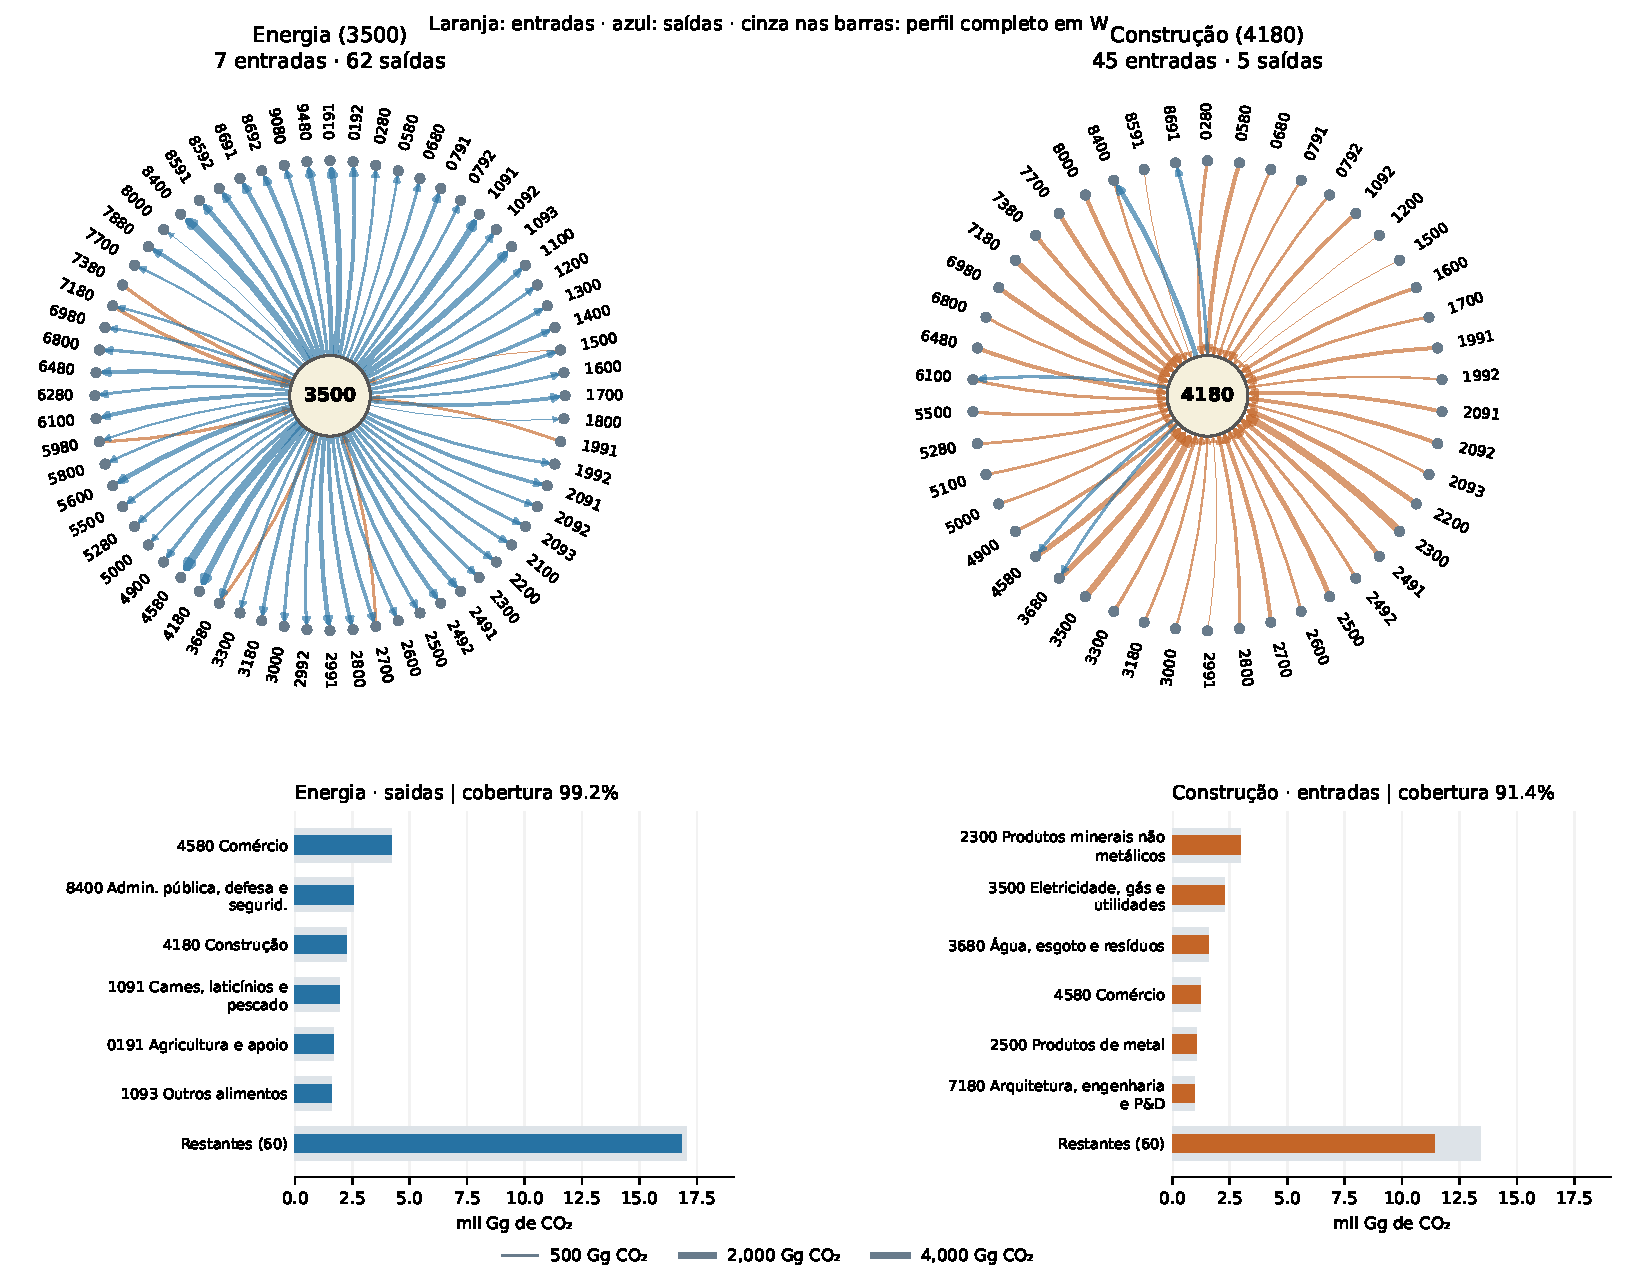
\includegraphics[width=\linewidth,height=0.55\textheight,keepaspectratio]{figuras/artigo_relacoes_combinada.pdf}
\caption{Contrapartes e cobertura dos perfis de energia e construção.}
\label{fig:relacoes-focais}
\begin{minipage}{\linewidth}\footnotesize
Fonte: elaboração própria. Acima: todas as relações incidentes a energia e construção no backbone de $\alpha=0{,}05$, sem diagonal; setas da origem emissora ao produto final. Azul: saídas; laranja: entradas; espessura proporcional à raiz do peso, com escala comum em Gg de CO\textsubscript{2}. Nós centrais identificam as atividades focais; demais códigos constam do Apêndice E. Posição circular sem interpretação econômica. Abaixo: saídas de energia e entradas de construção, com as seis maiores contrapartes em $W$ e soma das 60 restantes. Cinza: peso completo; cor: parcela retida, sem renormalização. Escala linear comum, em mil Gg de CO\textsubscript{2}. Cobertura relativa ao perfil inteiro. O agregado restante não representa uma atividade.
\end{minipage}
\end{figure}
%TC:endignore
